\documentclass[tikz, margin=3.14mm]{standalone}

\usepackage{tikz}
\usetikzlibrary{decorations, calc, arrows, arrows.meta, positioning}

\begin{document}
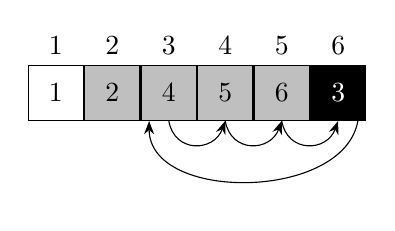
\begin{tikzpicture}[
    >=Stealth,
    array/.style={rectangle, draw, inner sep=5pt, text=black,
        minimum width = 20pt, minimum height = 20pt}
]

    % Nodes ------------------------------------------------------

    \node[array] (n1) {1};
    \node[array, right=0cm of n1, fill = lightgray] (n2) {2};
    \node[array, right=0cm of n2, fill = lightgray] (n3) {4};
    \node[array, right=0cm of n3, fill = lightgray] (n4) {5};
    \node[array, right=0cm of n4, fill = lightgray] (n5) {6};
    \node[array, right=0cm of n5, fill = black, text = white] (n6) {3};

    % labels
    \node[above=0cm of n1] (n1_label) {1};
    \node[above=0cm of n2] (n2_label) {2};
    \node[above=0cm of n3] (n3_label) {3};
    \node[above=0cm of n4] (n4_label) {4};
    \node[above=0cm of n5] (n5_label) {5};
    \node[above=0cm of n6] (n6_label) {6};

    % Arrows ---------------------------------------------------

    \draw [->] ($(n6.south)+(.25,0)$) to[out=-100, in=-90, looseness=1] ($(n3.south)-(.25,0)$);
    \draw [->] (n3.south) to[out=-80, in=-110, looseness=1.5] (n4.south);
    \draw [->] (n4.south) to[out=-80, in=-110, looseness=1.5] (n5.south);
    \draw [->] (n5.south) to[out=-80, in=-110, looseness=1.5] (n6.south);

\end{tikzpicture}
\end{document}